
\subsection{Descripción de alto nivel de la solución aportada}

Para la implementación del trabajo realizado, de cara a poder desarrollar las fases CIM y PIM de MDA en el ámbito seleccionado como ejemplo (el desarrollo de sintetizadores de audio software), se han implementado 4 DSLs en lenguaje Langium, y un IDE de desarrollo completo, ya mencionado en el apartado de introducción, llamado MDAA (Model-Driven Development Audio), que implementa estos 4 DSLs, y sirve de soporte para su generación.


\section{Descripción detallada de la solución propuesta}

En el repositorio del proyecto, se encuentra ampliamente documentada la definición de estos 4 DSLs desarrollados (véase Manual DSL\footnote{\href{\urlProyectoManualDsl}{Manual DSL en GitHub}}), por lo que el presente apartado se limitará a exponer las ideas clave detrás del diseño de los mismos.

\subsubsection*{Lenguajes de Análisis (CIM)}
\begin{itemize}
    \item \texttt{mdaa-cim-machine}: Permite la definición conceptual de máquinas de audio, estableciendo su identidad, puertos de comunicación y configuraciones base. Una máquina, concepto ampliamente expuesto en la documentación de los DSL, se puede considerar como un conjunto de elementos que interactuan entre si, pero que tienen una finalidad común, que es la finalidad de la máquina en su conjunto.
    \item \texttt{mdaa-cim-relations-machines}: Define las conexiones conceptuales y el flujo de señales, a nivel abstracto, entre las distintas máquinas definidas en el análisis.
\end{itemize}

\subsubsection*{Lenguajes de Diseño (PIM)}
\begin{itemize}
    \item \texttt{mdaa-pim-machine}: Facilita la definición detallada de la arquitectura interna de las máquinas, especificando generadores de audio, modificadores de los parámetros o señales de los generadores, y efectos de procesado de señales de audio.
    \item \texttt{mdaa-pim-relations-machines}: Se encarga de la orquestación de las interconexiones técnicas y vínculos detallados entre los componentes internos de las máquinas.
\end{itemize}

La idea clave de los DSL, centrados en el ámbito de creación de software para audio, pero extrapolables a cualquier otro ámbito, reside en dos puntos clave:

\begin{enumerate}
    \item Todo elemento, tanto de análisis como de diseño, debe tener una relación con algún otro.
    \item El análisis de un proyecto ya no puede ser un conjunto de textos que se relacionan semánticamente con los artefactos de diseño. Para que un modelo de razonamiento automático pueda trabajar de forma eficiente, el análisis debe estar estrictamente configurado, y sus relaciones deben ser explícitas.
\end{enumerate}

La herramienta desarrollada, MDAA (Model Driven Development Audio), imprescindible para que las gramáticas DSL desarrolladas resulten usables en desarrollos reales, se encuentra también ampliamente documentada en el repositorio del proyecto (véase Manual MDAA\footnote{\href{\urlProyectoManualMdaa}{Manual MDAA en GitHub}}). La idea clave de esta herramienta se puede resumir en los siguientes tres puntos:

\begin{enumerate}
    \item Debe servir para que un analista, especializado en el dominio de aplicación (el desarrollo de sintes de audio en este caso), trabajando sobre un alto nivel de abstracción, pueda ser capaz de entender e implementar los DSL CIM desarrollados.
    \item Debe servir para que un diseñador, especializado en el dominio de aplicación (sintetizadores de audio), trabajando ya en un nivel más bajo de abstracción, pueda ser capaz de entender e implementar los DSL PIM desarrollados.
    \item Debe proporcionar una forma sencilla de poder generar los artefactos necesarios para que un modelo de razonamiento automático pueda generar el código fuente requerido.
\end{enumerate}

\begin{figure}[H]
    \centering
    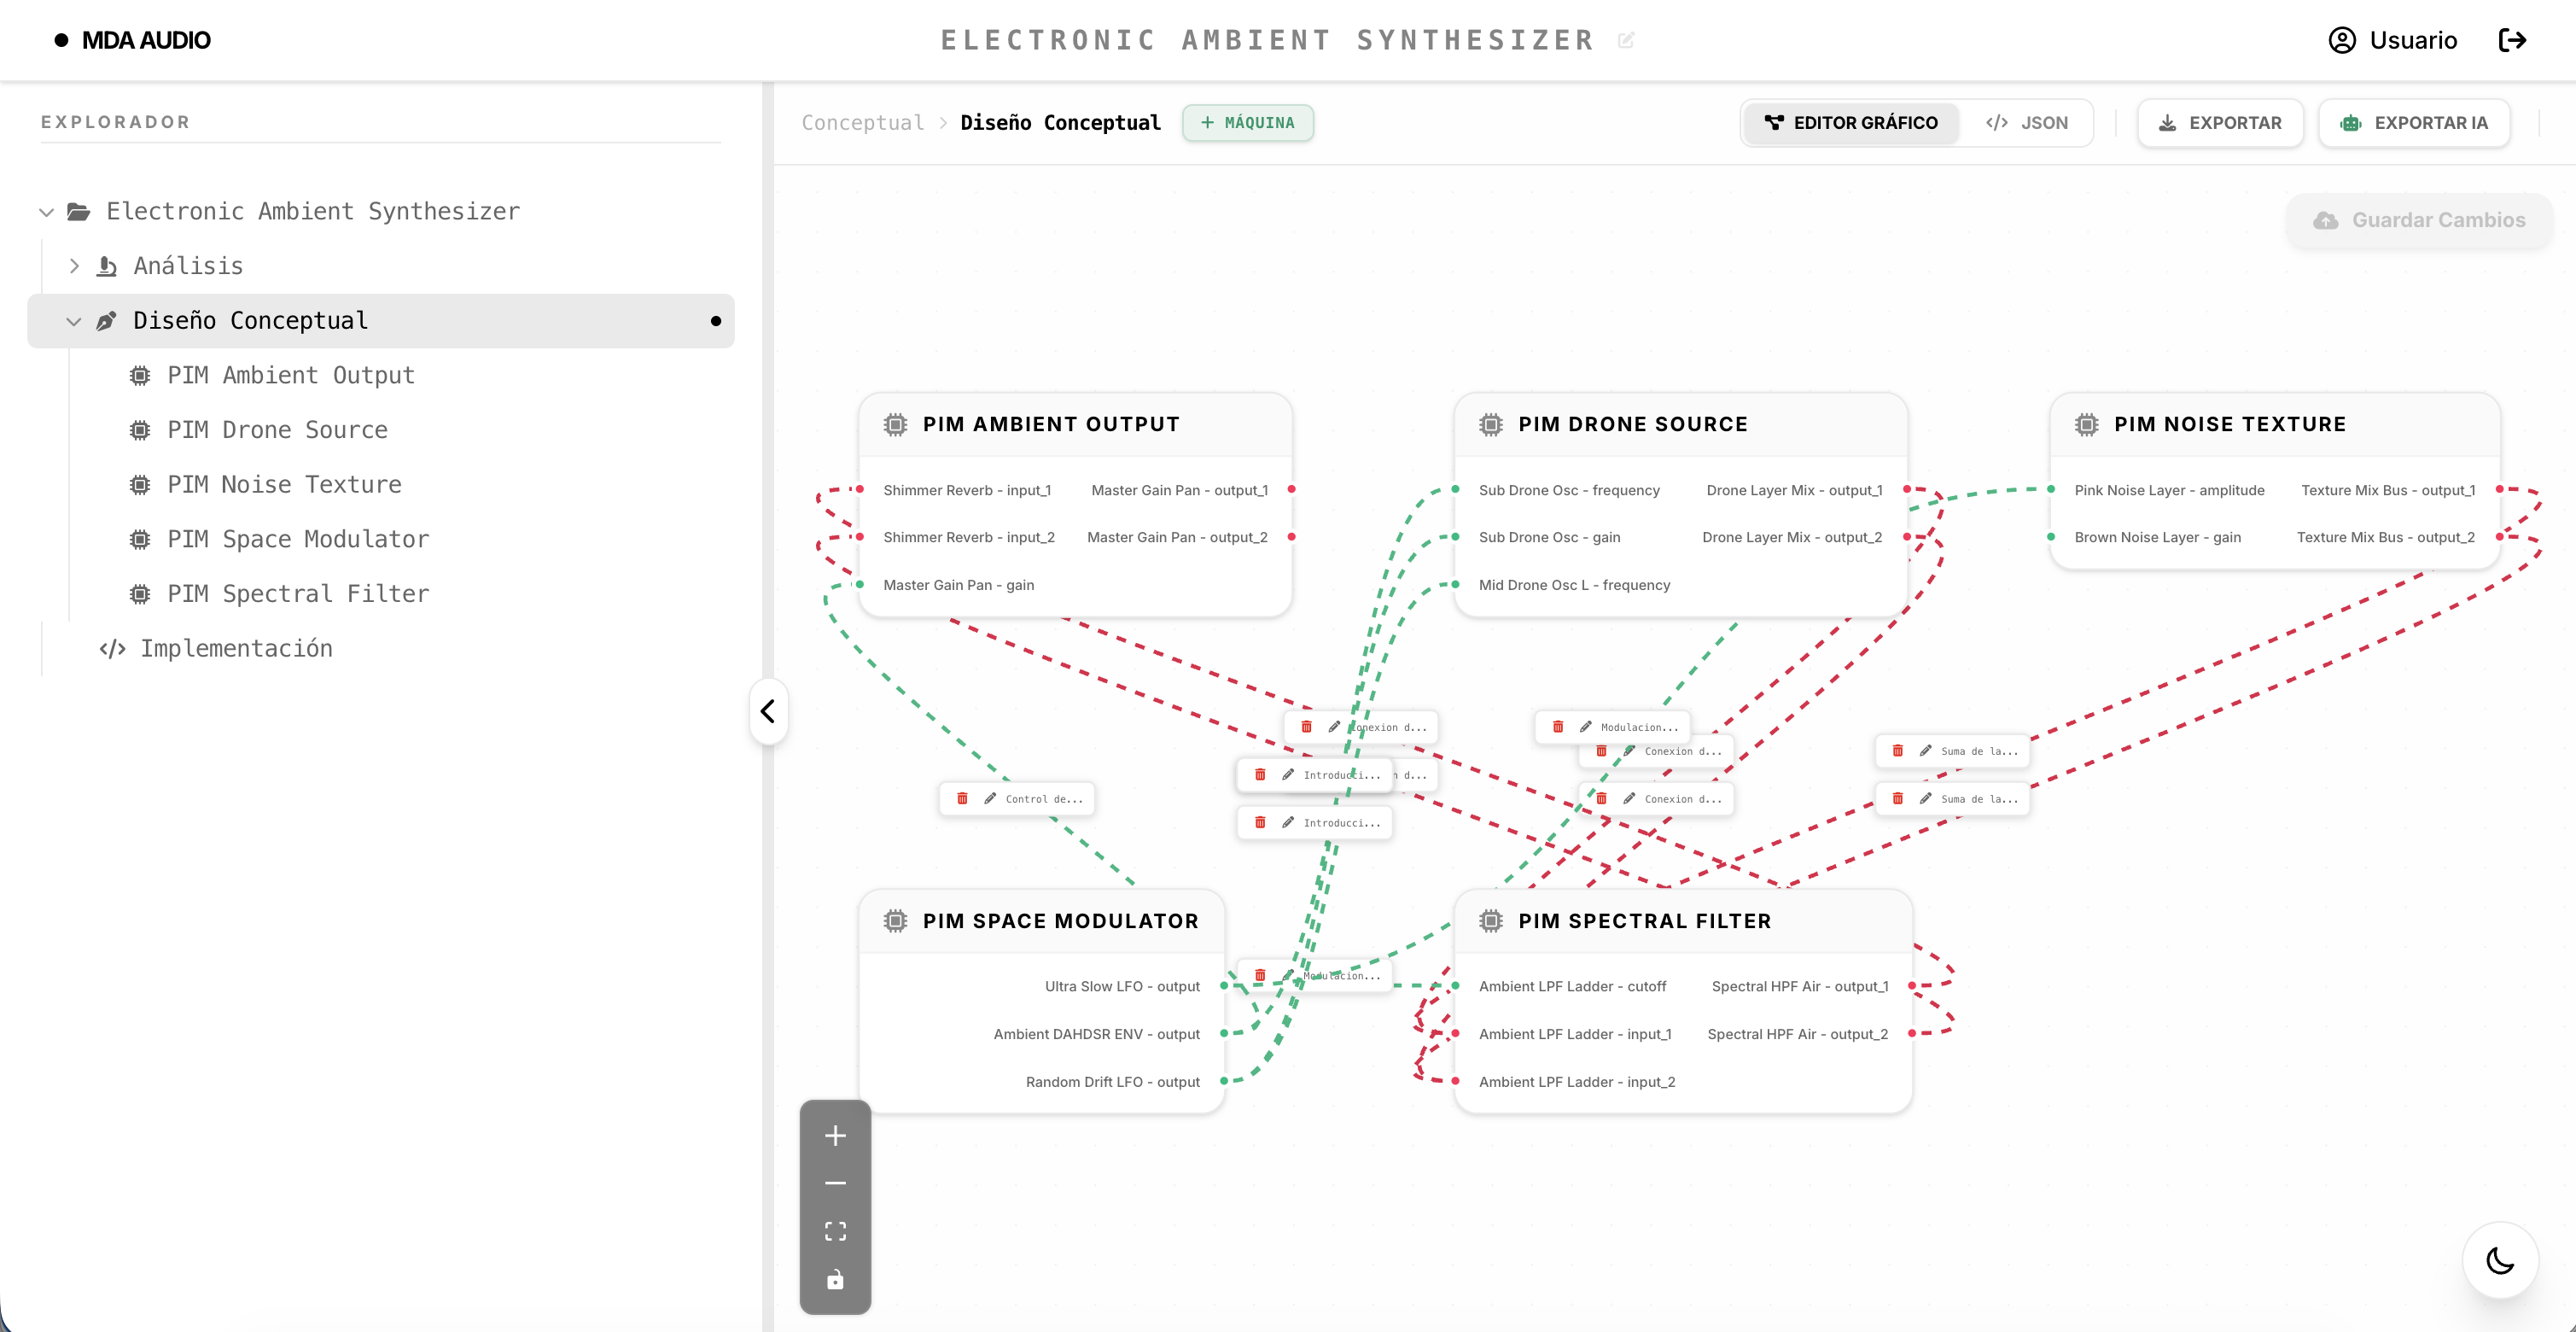
\includegraphics[width=\linewidth]{imagenes/01_pantallaDisenoConceptual.png}
    \caption{Relaciones entre máquinas, en el nivel de diseño conceptual (PIM), mediante la herramienta MDAA.}
    \label{fig:01_pantallaDisenoConceptual}
\end{figure}

\section{Descripción detallada de las herramientas generadas}

En el repositorio del proyecto (véase Repositorio en GitHub\footnote{\href{\urlProyecto}{Repositorio en GitHub}}), se incluye un fichero \texttt{README.md} que resume todo el trabajo realizado respecto de las herramientas implementadas y su uso. Esta guía también sirve como base para navegar por los distintos apartados, scripts ejecutables y manuales de las herramientas implementadas. Por otro lado, el código fuente tanto de los DSL como de la herramienta MDAA se encuentra exhaustivamente documentado, empleando el estándar Javadoc para el código desarrollado en Java (tecnología usada para el \textit{backend}) y JSDoc para las secciones implementadas en VUE/TypeScript (tecnología usada para el \textit{frontend}).

Para la ejecución local del proyecto MDAA, necesitaremos tener instalado docker compose. Como se podrá ver en el \textit{README.md} antes mencionado, tendremos una serie de scripts que facilitarán tanto la ejecución de la herramienta como la comprobación de los DSLs desarrollados, así como utilizades como el incluir los casos de uso en el entorno local instalado. Para ejecutarlos, se necesita una terminal linux-like (como puede ser la terminal de Linux, WSL de Windows, o la terminal de MacOS). Para la ejecución, compilación y validación de los DSL, como del script \texttt{validar-test.sh} (también comentado en el \textit{README.md} antes mencionado), se necesita tener instalado nodejs. 



\subsection{Casos de uso aplicados para las pruebas de demostración.}

En la carpeta de casos de prueba del repositorio del proyecto (véase Casos de Prueba\footnote{\href{\urlProyectoCasosPrueba}{Casos de Prueba en GitHub}}), se encuentran documentados todos los casos de prueba realizados para la evaluación de la solución aportada. También se incluye un fichero \textit{README.md}, comentando sus usos y formas de validación.